\section{Update phase}



  As in the fwd-bwd case, we will describe the details of the
  algorithm for the case of 3D images.
  \subsection{Serial algorithm}

  Similarly as in the fwd-bwd case, we first divide the algorithm into
  primitives that compute $S^2$ convolutions of $S$ input images with
  $S$ gradients.

  We implement the following algorithm described in
  Algorithm~\ref{alg:serial-update-subtask} that computes a
  convolution of an $R_F$ images of size $R_D \times R_H \times (W + R_W
  - 1)$ by $S$ images of size $1 \times 1 \times W$ separately, to
  produce and accumulate the results of $R_F \times S$ images of size
  $R_D \times R_W \times R_H$.

  \begin{algorithm}
    {\footnotesize
      \begin{codebox}
        \Procname{$\proc{Update-Subtask} \langle R_D, R_H, R_W, W, R_F \rangle(a,b,r)$}
        \li \kw{simd register} $oreg[R_D][R_H][R_W][R_F]$
        \li \kw{simd register} $wreg$
        \li $oreg[:][:][:][:][:] \gets \proc{LOAD}(r[:][:][:][:][:])$
        \li \For $i \gets 0 \To W-1$ \Comment Partially unrolled
        \li   \Do $wreg \gets \proc{LOAD}(b[1][1][w][:])$
        \li   \For $d \gets 0 \To R_D-1$ \Comment Fully unrolled
        \li   \Do \For $h \gets 0 \To R_H-1$  \Comment Fully unrolled
        \li   \Do \For $w \gets 0 \To R_W-1$  \Comment Fully unrolled
        \li       \For $f \gets 0 \To R_F-1$   \Comment Fully unrolled
        \li   \Do $oreg[d][h][w][f] \gets \proc{FMADD}($
        \li   \Do $wreg,$
        \li       $\proc{EXLOAD}(a[d][h][w+i][f]),$
        \li       $oreg[d][h][w][f])$
        \End
        \End \li \kw{end for} $f$
        \End \li \kw{end for} $w$
        \End \li \kw{end for} $h$
        \End \li \kw{end for} $d$
        \End \li \kw{end for} $i$
        \li $r[:][:][:][:][:] \gets \proc{STORE}(oreg[:][:][:][:][:])$
      \end{codebox}
    \caption{Serial update subtask.}
    \label{alg:serial-update-subtask}
    }
  \end{algorithm}

  The algorithm relies on the compiler to use register file, and
  unroll loops.  In order for that to be possible, the $oreg$ and
  $wreg$ variables have to fit in the register file.  That means that
  $R_D \times R_H \times R_W \times R_F + 1 \le R$, where $R$ is the
  number of vector registers available to the system.  Note how most
  of the computation involves FMADD instructions with the arguments
  either in the register file, or in $L1$ cache.

  Performing a convolution of $S$ images of size $K_D \times K_H
  \times K_W \times (W+K_W-1)$ with $S$ images of size $1 \times 1
  \times W$ can be performed by computing $R_D \times R_H \times R_W$
  results of $S \times R_F$ results using the algorithm described
  above.  We prefer decompositions for which the values of $R_D \times
  R_H \times R_W \times R_F$ are large, but smaller than $R$.  Out of
  different combinations we prefer ones for which $R_F$ is maximized,
  then $R_W$ is maximized, and so on.

  We would like to use at least half of the available registers, which
  can be always accomplished by choosing $R_F = S$, as for all
  architectures $S = R/2$.  However, better solutions might exist.  We
  find the best solution during compile time using C++ meta
  programming.  The solution has to divide the computed values evenly
  (into subsets of the same size).  For example, on AVX512 machine,
  where $R=32$, $S=16$, for a kernel of size $2 \times 3 \times 3$
  (VD2D3D) we get a decomposition into $R_D=R_H=1$, $R_W=3$ and
  $R_F=8$.  This uses 24 of the available registers.

  The computation is performed by sliding $R_D \times R_H \times R_W
  \times R_F$ first over the output images, then the least significant
  dimension, and so on.

  %% \begin{algorithm}
  %%   {\footnotesize
  %%     \begin{codebox}
  %%       \Procname{$\proc{Update-Task} \langle I_D, I_H, I_W, O_D, O_H, O_W \rangle(a,b,r)$}
  %%       \li $\angled{K_D,K_H,K_W} \gets \angled{I_D-O_D+1,I_H-O_H+1,I_W-O_W+1}$
  %%       \li $\angled{R_D,R_H,R_W,R_F} \gets \proc{Decompose}(K_D,K_H,K_W,S)$
  %%       \li \For $d \gets 0 \To O_D-1$
  %%       \li   \Do \For $h \gets 0 \To O_H-1$
  %%       \li     \Do \For $r_d \gets 0 \To K_D/R_D-1 \kw{ by } K_D/R_D$
  %%       \li       \Do \For $r_h \gets 0 \To K_H/R_H-1 \kw{ by } K_H/R_H$
  %%       \li          \Do \For $r_w \gets 0 \To K_W/R_W-1 \kw{ by } K_W/R_W$
  %%       \li            \Do \For $r_f \gets 0 \To S/R_F-1 \kw{ by } S/R_F$
  %%       \li \Do $\proc{Update-Subtask}\langle R_D,R_H,R_W,O_W,R_F\rangle ($
  %%       \li \Do $a[d+r_d,R_D][h+r_h,R_H][r_w,O_W][:],$
  %%       \li     $b[d][h][:][r_f,R_F],$
  %%       \li     $r[r_d,R_D][r_h,R_H][r_w,R_W][r_f,R_F][:])$
  %%       \End
  %%       \End \li \kw{end for} $r_f$
  %%       \End \li \kw{end for} $r_w$
  %%       \End \li \kw{end for} $r_h$
  %%       \End \li \kw{end for} $r_d$
  %%       \End \li \kw{end for} $h$
  %%       \End \li \kw{end for} $d$

  %%     \end{codebox}
  %%   \caption{Serial update task.}
  %%   \label{alg:serial-update-task}
  %%   }
  %% \end{algorithm}

  \begin{figure}
    \begin{center}
      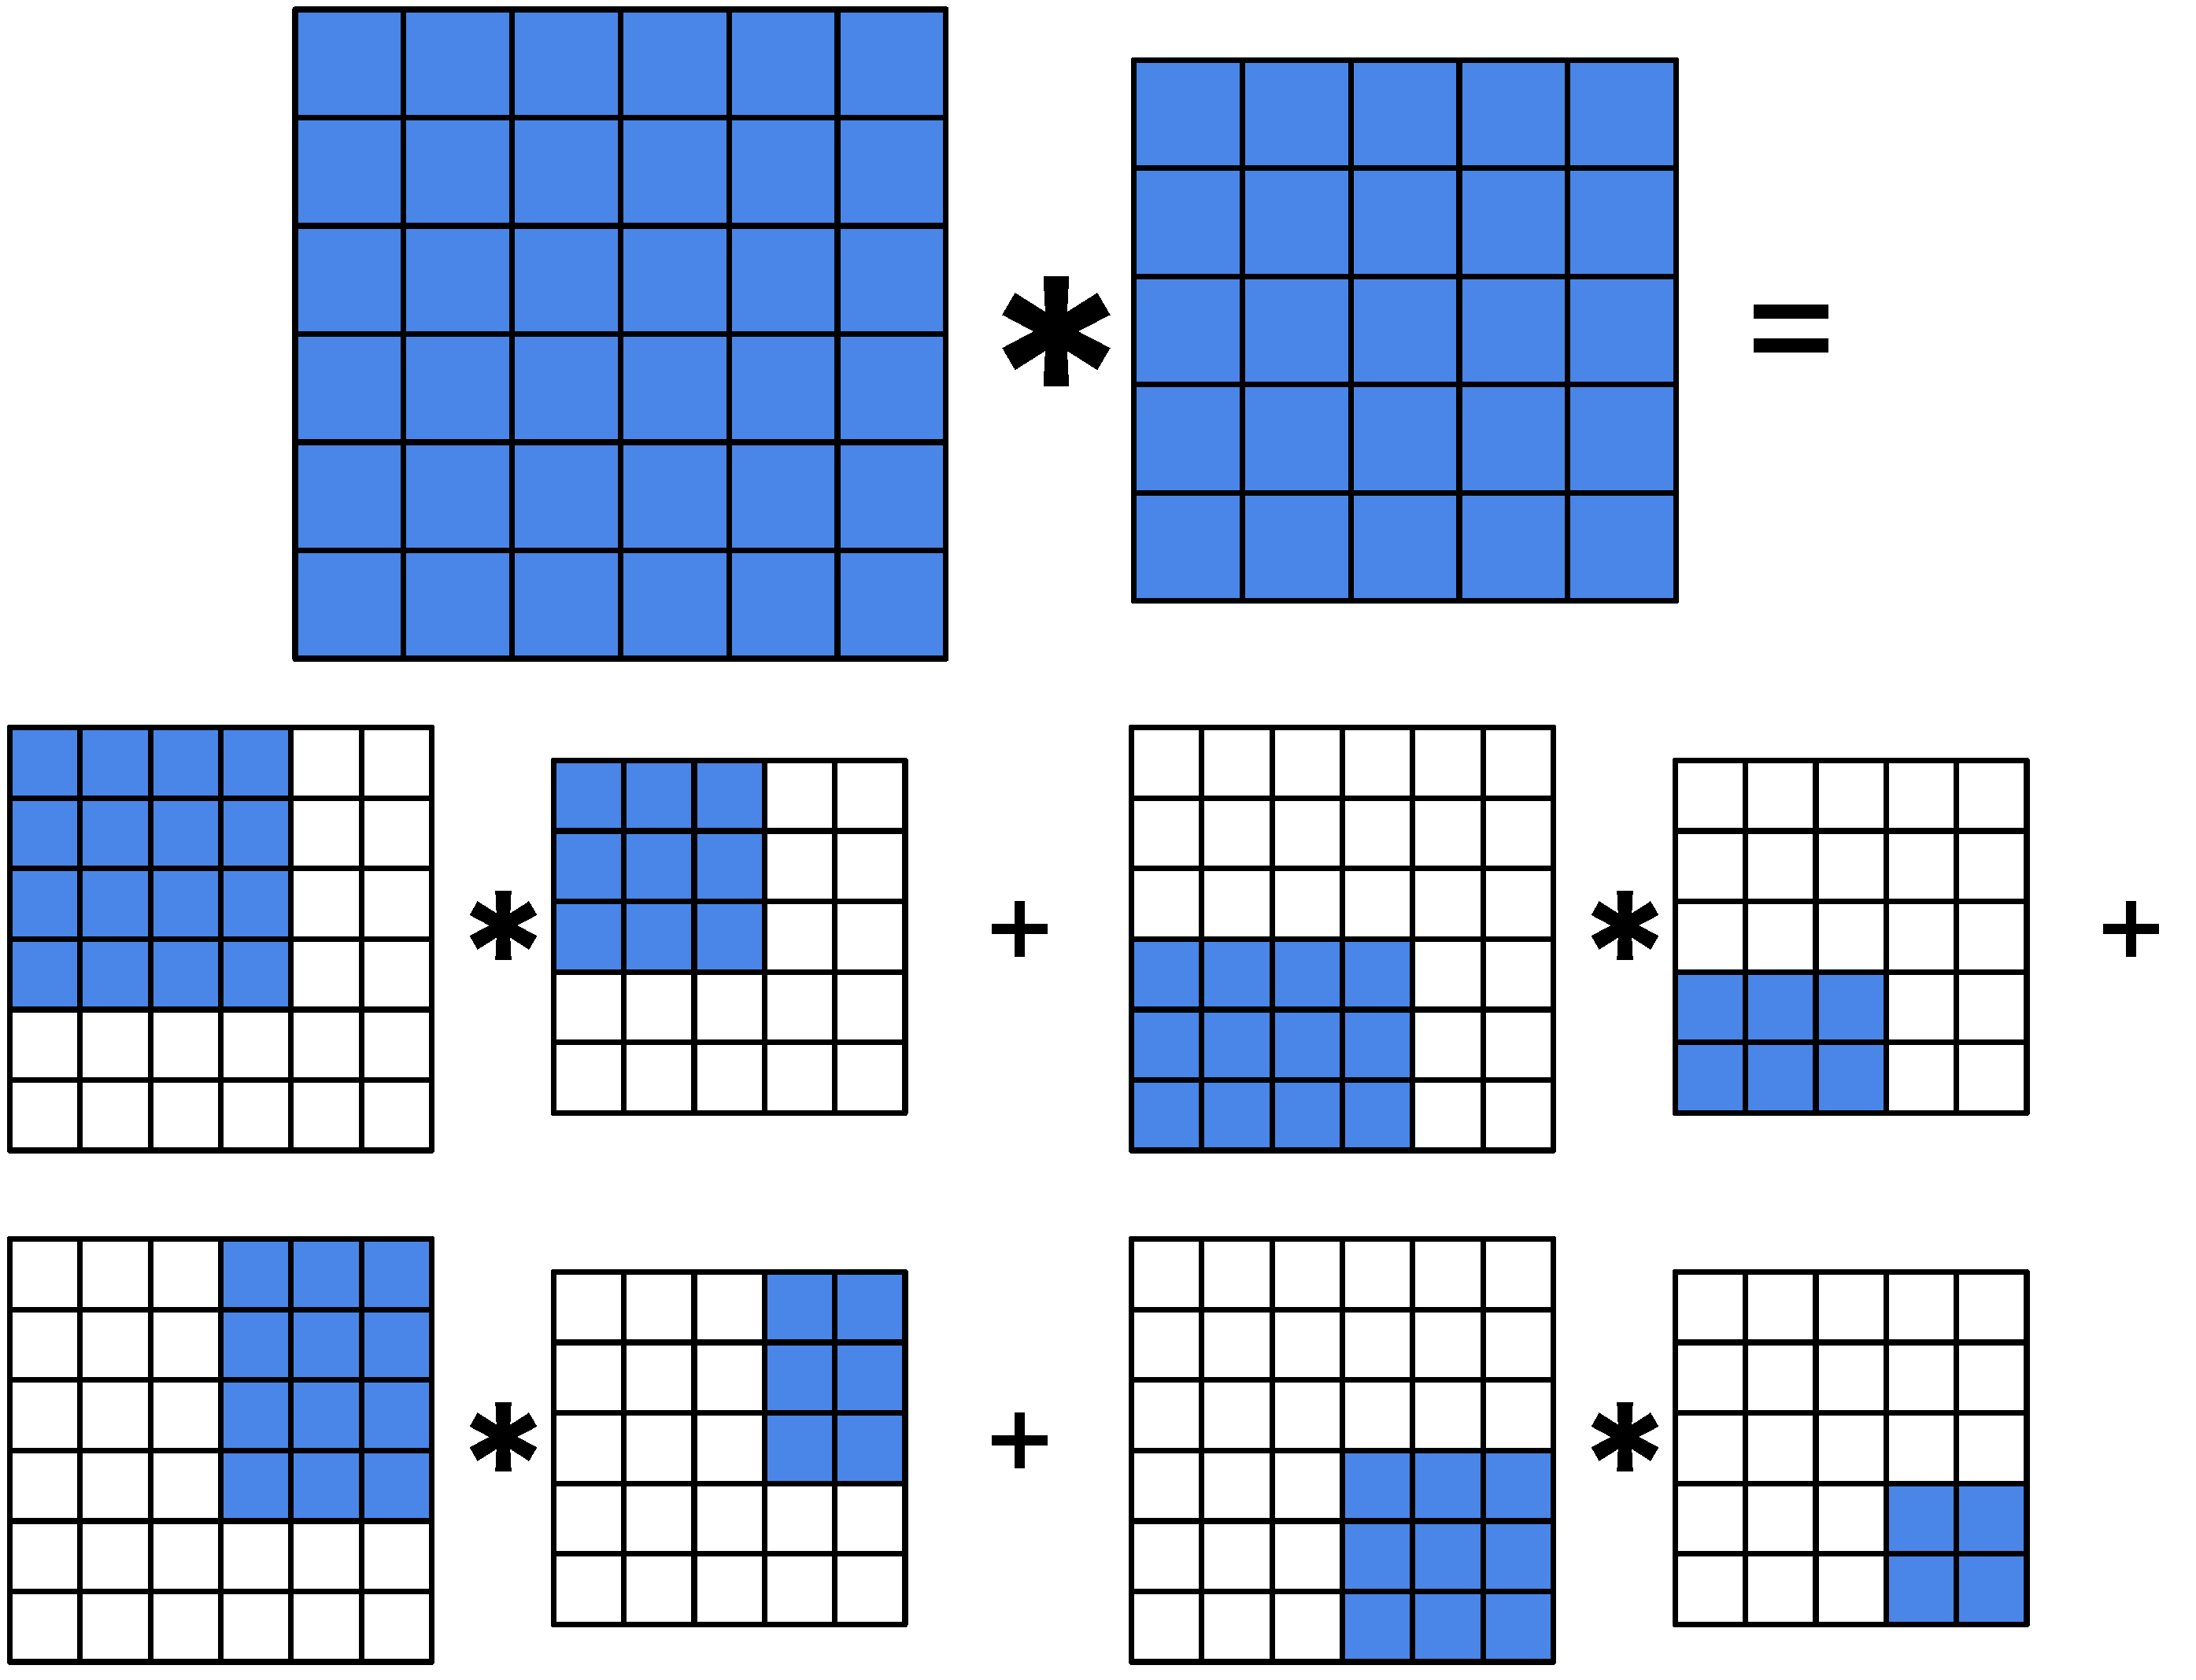
\includegraphics[width=0.67\linewidth]{fig/decomposition}
    \end{center}
    \caption{Decomposing a convolution.}
    \label{fig:conv-decomposition}
  \end{figure}



  \aleks{Explain why and how}.




  \subsection{Parallel execution}
